%% LyX 2.3.7 created this file.  For more info, see http://www.lyx.org/.
%% Do not edit unless you really know what you are doing.
% \documentclass[english]{amsart}
\documentclass[12pt,reqno]{book}
% \usepackage[T1]{fontenc}
% \usepackage[latin9]{inputenc}
\usepackage{amstext}
\usepackage{amsthm}
\usepackage{amsmath}
\usepackage{xcolor}
\usepackage{graphicx}
\usepackage{setspace}
\usepackage{float}  

\setstretch{1.15} 

% Statement
% Arc Length
% Pendulum
% Spring Pendulum
% Proof

\newtheorem{theorem}{Theorem}
\makeatletter
%%%%%%%%%%%%%%%%%%%%%%%%%%%%%% Textclass specific LaTeX commands.
% \numberwithin{equation}{section}
% \numberwithin{figure}{section}

\makeatother

% \usepackage{babel}
\begin{document}

\begin{center}
{\bf The Euler-Lagrange Equation}

\indent {\bf By Charlie Kim}

\end{center}

\noindent{\bf Abstract}
%Find a function $x(t)$ that extremizes the functional $L$.
This review paper aims to derive and provide examples for the Euler-Lagrange equations, fundamental equations both in physics and the calculus of variations. 

Here we are going to outline the proof of the Euler Lagrange equation.

\medskip


\noindent{\bf The Euler-Lagrange Equation Proof}

The following is a formal statement of the Euler-Lagrange equation.

\begin{theorem}\label{thm:EL}
    Let $J$ be the functional\textsuperscript{1} defined by \[J[f] := \int_{t_{1}}^{t_{2}}L(t,f(t),f'(t))\] with an extremum on the interval $[t_1,t_2]$. Let $x(t)$ be a $C^1[t_1,t_2]$ function that extremizes $J$. Then the following equation must be satisfied: 


    \begin{align*}
        \frac{d}{dt} \cdot \frac{\partial L}{\partial\dot{x}} = \frac{\partial L}{\partial x}.
    \end{align*}
    
\end{theorem}

Recall that $C^1[a,b]$ represents the set of all functions that have a continuous derivative on $(a,b)$. Recall from Calculus every differentiable function is continuous.

\begin{proof}


By assumption in the Theorem~\ref{thm:EL}, let $x \in C^1[t_1,t_2]$ be a function that extremizes $J$. We wish to show that 
\begin{align*}
    \frac{d}{dt} \cdot \frac{\partial L}{\partial\dot{x}} = \frac{\partial L}{\partial x}.
\end{align*}

% For a functional J with an extremum on the interval $[t_1 , t_2]$ such that: 
% $$J(a) = \int_{t_{1}}^{t_{2}}f(x(t),\dot{x}(t),t)dt, $$
%     we wish to find the function $x(t)$ that extremizes J.

  Let $A(t)$ be an arbitrary function and $A(t_{1})=A(t_{2})=0$. 
 Therefore any function in $C^1[t_1 , t_2]$ can be represented with 
 \begin{align*}
    x(t,a) = x(t) + aA(t)
 \end{align*}
 where x(t,a) is a combination x(t), our function that extremizes J, and A(t), the "divergence" from that function, parameterized by a. 
    

Let $$J(a) = \int_{t_{1}}^{t_{2}}f(x(t,a),\dot{x}(t,a),t)dt, $$ be functional
parameterized by $a$. 


Note when $a = 0$, x(t,a) becomes x(t). Thus when $a = 0$ J has an extremum by defintion of x(t) and  $$\frac{dJ}{da}\biggr\vert_{a=0} =0.$$ 


$$\frac{dJ}{da}=\frac{d}{da}\int_{t_{1}}^{t_{2}}f(x(t,a),\dot{x}(t,a),t)dt$$ 

So, by the chain rule, we have
\begin{align*}
0=\int_{t_{1}}^{t_{2}}\frac{\text{\ensuremath{\partial f}}}{\partial x}\frac{\partial x}{\partial a}+\frac{\text{\ensuremath{\partial f}}}{\partial\dot{x}}\frac{\partial\dot{x}}{\partial a}dt.
\end{align*}


Solving for  $\frac{\partial x}{\partial a}$ and $\frac{\partial \dot{x}}{\partial a}$ we get 

\begin{align*}
    \frac{\partial x}{\partial a} & =A(t)\\
    \frac{\partial\dot{x}}{\partial a} & =\frac{\partial x}{\partial a}\cdot\frac{d}{dt}=A'(t)
\end{align*}


\[
0=\int_{t_{1}}^{t_{2}}\frac{\text{\ensuremath{\partial f}}}{\partial x}\cdot A(t)+\frac{\text{\ensuremath{\partial f}}}{\partial\dot{x}}\cdot A'(t).
\]

Using Integration by parts: 
\begin{align*}
\int\frac{\text{\ensuremath{\partial f}}}{\partial\dot{x}}\cdot A'(t)dt & =\frac{\partial f}{\partial\dot{x}}A(t)\bigr\vert_{t_{1}}^{t_{2}}-\int\frac{d}{dt}\cdot\frac{\text{\ensuremath{\partial f}}}{\partial\dot{x}}*A(t)dt\\
 & =-\int\frac{d}{dt}\cdot\frac{\text{\ensuremath{\partial f}}}{\partial\dot{x}}*A(t)dt
\end{align*}

Thus the equation becomes,
\begin{align*}
0 & =\int_{t_{1}}^{t_{2}}\frac{\text{\ensuremath{\partial f}}}{\partial x}\cdot A(t)-\frac{d}{dt}\frac{\text{\ensuremath{\partial f}}}{\partial\dot{x}}\cdot A(t)dt\\
 & =\int A(t)\cdot(\frac{\partial f}{\partial x}-\frac{d}{dt}\cdot\frac{\partial f}{\partial\dot{x}})dt
\end{align*}

As $A(t)$ is arbitrary, by the fundamental lemma of calculus of variations (appendix):
\begin{align*}
\frac{\partial f}{\partial x}-\frac{d}{dt}\cdot\frac{\partial f}{\partial\dot{x}} & =0\\
\frac{d}{dt}\cdot\frac{\partial f}{\partial\dot{x}} & =\frac{df}{dx}
\end{align*}

proving Euler's equation.   This equation must be satisfied for a function
x(t) that extremizes the functional L.  

\medskip
\noindent{\bf Arc-Length}

An immediate consequence of the Euler-Lagrange equation is the classical 
fact that the shortest distance between two points is a straight line. We will 
show this derivation now.
\begin{theorem}\label{thm:arc-length}
Let $a$ and $b$ be two real numbers with $a < b$. Let $c$
and $d$ be two arbitrary real numbers. Then the unique differentiable function $x(t)$, with $x(a) = c$ and $x(b) = d$, that extremizes the functional
\[
S(x)=\int_a^b \sqrt{1+(\frac{dx}{dt})^{2}}dt. 
\]
is the linear function $x(t) = mt + y_0$ for some real numbers $m$ and $y_0$.
\end{theorem}




% This is the functional that calculates the arc length of a given path.

\noindent\begin{proof}

Let $x(t)$ be the function that extremizes $S(x)$.  

The integrand in $S$ can be represented by a functional L, 
\[L(t,x,x') = \sqrt{1+(\dot{x})^{2}}.\]

We know from Theorem~\ref{thm:EL} (Euler Lagrange Equation) and the fact that $x$ minimizes $S$, that 
\[\frac{dL}{dx} = \frac{d}{dt}\frac{dL}{d\dot{x}}.\]
Since $x$ is not present on in $L(t,x,\dot{x})$, we have
\[\frac{dL}{dx} = 0.\]
So we have 

% \text{The quotient rule} \\
% \text{The Chain Rule gives:} \\

\begin{align*}
    0 &= \frac{d}{dt}\frac{dL}{d\dot{x}} \\
    &=  \frac{d}{dt}\frac{\dot{x}}{\sqrt{1+(\dot{x})^{2}}}\\
 & = \frac{\ddot{x}\sqrt{1+(\dot{x})^{2}}-\dot{x}^{2}\ddot{x}(1+\dot{x})^{-\frac{1}{2}}}{1+(\dot{x})^{2}}\\ 
& = \frac{\ddot{x}}{(1+\ddot{x}^{2})^{\frac{3}{2}}}.
\end{align*}
In the second inequality we used the quotient rule from Calculus and in the third line we used the chain rule.
Thus $\ddot{x}$ must be 0 
$$\ddot{x}  =0 ,$$
on the interval $(a,b)$. By a consequence of Rolle's theorem, $\ddot{x} =0$, $\dot{x}$ is a constant, say $m$. Therefore x has a constant slope and 

\[
x(t)  =mt+y_0,
\]
which is the equation for a line.


\end{proof}

We can solve for m and $y_0$, 
To solve for $m$ we use the rise over run for the interval $$m := \frac{x(a)-x(b)}{a-b} ,$$
then we can solve for $y_0$, given the point $(a,x(a))$ and $m$. 


Thus, the shortest distance between two points is a straight line. 

\medskip

\noindent{\bf Pendulum}



\begin{figure}[H]
    \centering
    {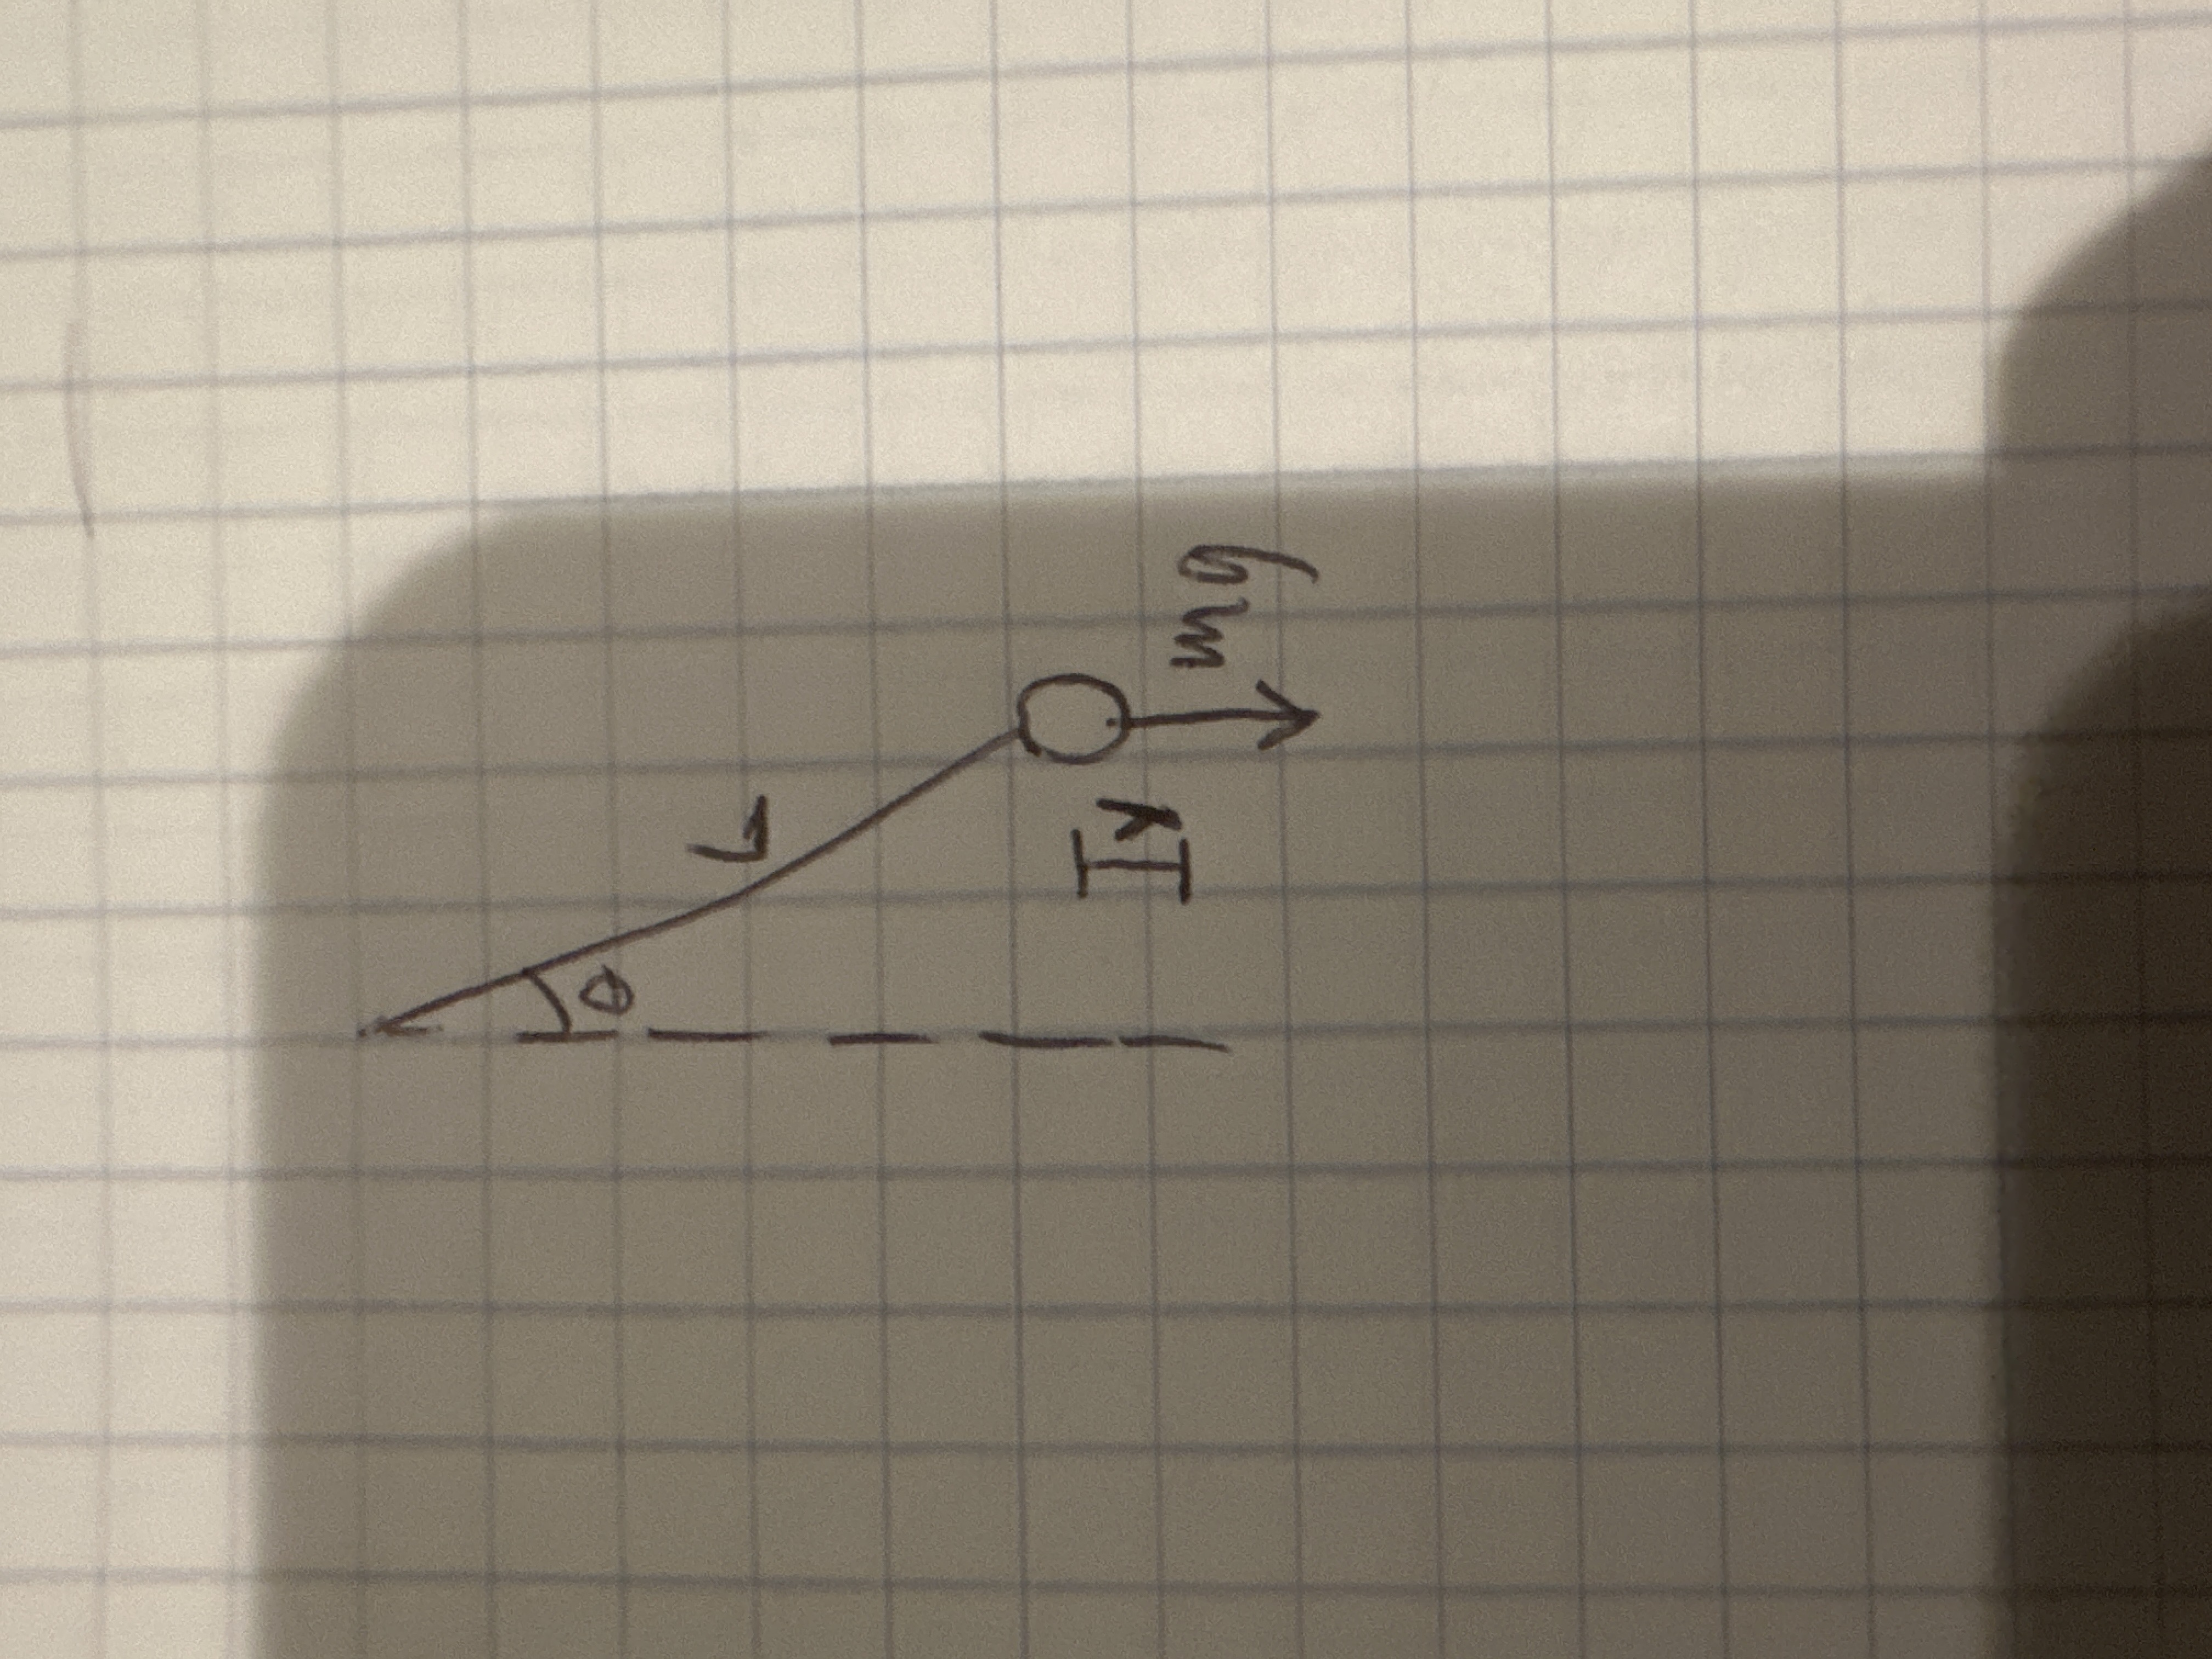
\includegraphics[width=0.4\textwidth]{images/IMG_2187.JPG}}
    \caption{Pendulum system}
    \label{fig:example_image}
\end{figure}

\noindent The potential energy of the system is 
$$
U = mgy = mg(l-lcos(\theta)).
$$
\noindent The kinetic energy is
$$
T = \frac{1}{2}m (v_{tangential})^2 = \frac{1}{2}m (l \dot{\theta})^2.
$$
\noindent Therefore our Lagrangian becomes
$$
L = T-U = \frac{1}{2}m (l \dot{\theta})^2-mg(l-lcos(\theta)).
$$
\noindent To find the equation of motion\textsuperscript{2} we use the Euler-Lagrange equation
\begin{align*}
    \frac{d}{dt}\frac{dL}{d\dot{\theta}}=\frac{dL}{d\theta}\\
    \frac{d}{dt} m l^2 \dot{\theta} = -m gl sin(\theta)\\
    \ddot{\theta} = -\frac{g}{l}sin(\theta)
\end{align*}
This equation of motion is a non-linear differential equation and is hard to solve. 
We can linearize the equation by using the approximation that
for small $\theta$ ($<20^\circ$), $\text{sin}(\theta) \approx \theta$. 
\begin{align*}
    \frac{d^2\theta}{dt^2} = \frac{g}{l}\theta
\end{align*}
Solving for theta we get (see Appendix)\textcolor{red}{Do I want to add calculation?}: 
\[
\theta = asin(\sqrt{\frac{g}{l}}t + b)
\]
Using a computer to model this, Euler approximations gives the following graph: 
\begin{figure} [H]
    \centering
    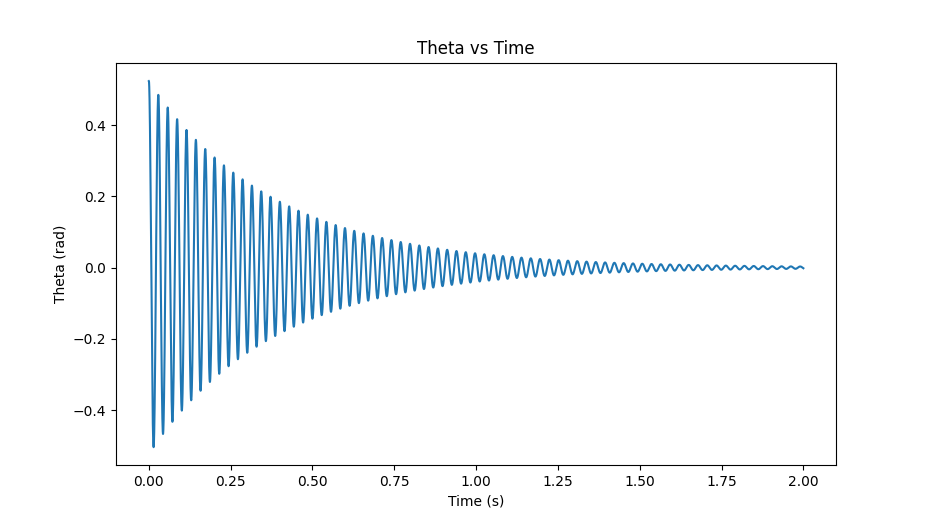
\includegraphics[width=1\linewidth]{images/graph.png}
    \caption{Euler Approximation}
    \label{fig:enter-label}
\end{figure}
1

\noindent{\bf Spring pendulum}

\begin{figure}[H]
    \centering
    \sc{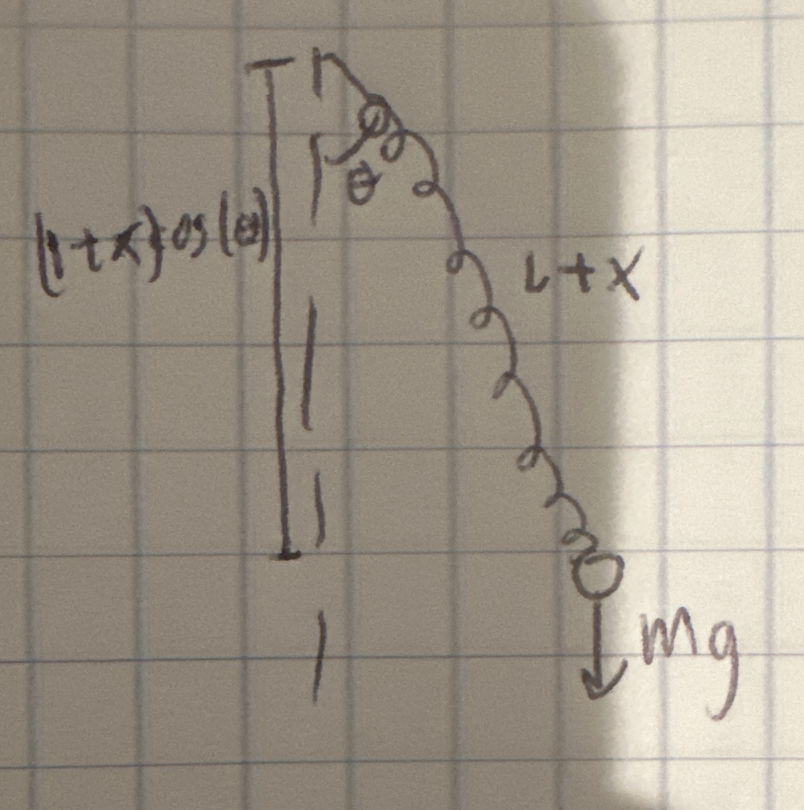
\includegraphics[width=0.4\textwidth]{images/spend.png}}
    \caption{Pendulum system}
    \label{fig:example_image}
\end{figure}
The potential energy of the system is a combination of the gravitational potential and the 
spring potential. 
\[
U=mg(l+x -(l+x)\cos(\theta))+\frac{1}{2}kx^{2}
\]
The Kinetic energy of the system is the linear kinetic energy of the
spring and the tangential Kinetic energy. 
\[
T=\frac{1}{2}m\dot{x}^{2}+\frac{1}{2}m(l+x)^{2}\dot{\theta}^{2}
\]
\noindent The Lagrangian is the kinetic minus potential energy
\[
L=T-U.
\]
This yields 
\[
L = \frac{1}{2}m(((l+x)\dot{\theta})^2 + \dot{x}^2)-mg(l+x)(1-cos(\theta)) - \frac{1}{2}kx^2
\]
To find the equation of motion with respect to x, we use
\begin{align*}
 \frac{d}{dt}\frac{dL}{d\dot{x}} & =\frac{dL}{dx}\\
 m\ddot{x} & = m(l+x)\dot{\theta}^{2}-mg(1-cos(\theta))-kx
\end{align*}
The LHS is the ma part of Newtons second law and the RHS is the gravitational
tangential force, the spring force, and the centrifugal force. 
To find the angular equation of motion we use the Euler-Lagrange equation with respect 
to $\theta$ 

\begin{align*}
 & \frac{d}{dt}\frac{dL}{d\dot{\theta}}=\frac{dL}{d\theta} \\ 
 & \frac{d}{dt}m(l+x)^2 \dot{\theta} = mg(l+x)sin(\theta)\\
 & m(l+x)^{2}\ddot{\theta} + 2m(l+x)\dot{x}\dot{\theta}=-mg(l+x)sin(\theta) \\
 & m(l+x)\ddot{\theta} + 2m\dot{x}\dot{\theta} = -mgsin(\theta)
\end{align*}

This equation is the torque equation $ma = T$ with the addition of the Coriolis force $2m\dot{x}\dot{\theta}$. 


\end{proof}
%\newpage
\noindent{\bf Appendix}

{\bf Definitions}

1. Functional: A functional takes in a function as the input and outputs a real number. 

2. equations of motion: differential equations that describe the dynamics of a system

{\bf Fundamental Lemma of Calculus of Variations}

Let $y(t)$ be  $C^1[t_1,t_2]$ and g(t) $\in C^2[t_1,t_2] $ such that $g(t_1)=g(t_2)=0$

\[
\int^{t_2}_{t_1} y(t)g(t)dt = 0
\]


\noindent Then $y(t) = 0 $ for $t_1 < t < t_2$
 

% \begin{align*}
    
% \end{align*}

\center\bf Works Cited

Gross, Jonathan. Principle of Least Action with Derivation. MIT, \url{https://web.mit.edu/~jgross/Public/least_action/Principle%20of%20Least%20Action%20with%20Derivation.html}{https://web.mit.edu/~jgross/Public/least_action/Principle\%20of\%20Least\%20Action\%20with\%20Derivation.html}.
"Euler–Lagrange Equation." Wikipedia, Wikimedia Foundation, \href{https://en.wikipedia.org/wiki/Euler–Lagrange_equation}{https://en.wikipedia.org/wiki/Euler–Lagrange\_equation}.  
Noubir, Teddy. Teddy Rocks Maths Essay. Tom Rocks Maths, 2021, \href{https://tomrocksmaths.com/wp-content/uploads/2021/05/teddy_rocks_maths_essay.pdf}{https://tomrocksmaths.com/wp-content/uploads/2021/05/teddy\_rocks\_maths\_essay.pdf}.  
Morin, David. Classical Mechanics: Chapter 6. Harvard University, \href{https://scholar.harvard.edu/files/david-morin/files/cmchap6.pdf}{https://scholar.harvard.edu/files/david-morin/files/cmchap6.pdf}.  
Feynman, Richard P. The Feynman Lectures on Physics Vol. II Chapter 19: The Principle of Least Action. Caltech, \href{https://www.feynmanlectures.caltech.edu/II_19.html\#:~:text=“In\%20other\%20words\%2C\%20the\%20laws,from\%20one\%20point\%20to\%20another.}{https://www.feynmanlectures.caltech.edu/II\_19.html\#:~:text=“In\%20other\%20words\%2C\%20the\%20laws,from\%20one\%20point\%20to\%20another.}




\end{document}
